\begin{figure*}[thp]
	\center
	\begin{subfigure}{0.7\textwidth}
		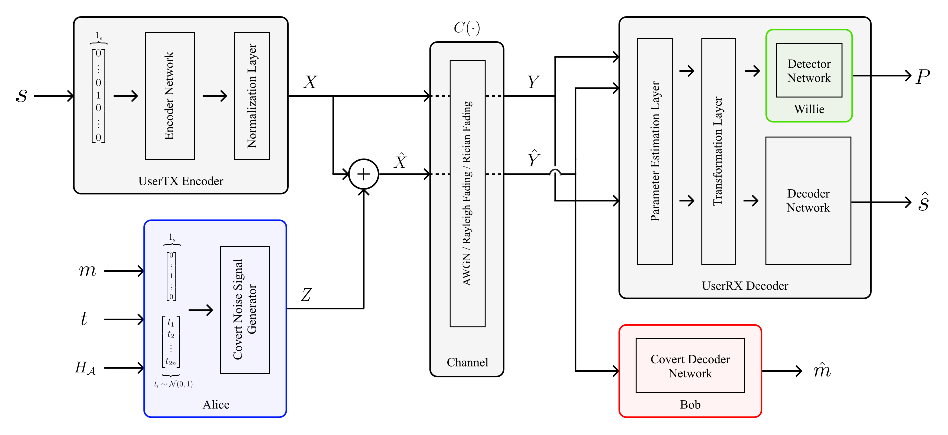
\includegraphics[width=\linewidth]{figs/system_architecture}
	\end{subfigure}
	\\
	\caption{Overall architecture of our system model in the single-user scenario. UserTX uses an encoder network to encode binary messages to a vector of signals and Alice perturbs them using her covert signals. After pass through the channel, UserRX extracts the normal message, Bob decodes the covert message, and Willie tries to distinguish covert and normal signals from the signals. (Colored components are under the control of covert users and gray components are the non-controllable parts of the system)}	
	\label{fig:system_architecture}
\end{figure*}


\section{System Model}
\label{s:single-model}
In this section, we provide an overview of the system and define each actor's rule in our system model.


Our system consists of two groups of users. The first group is the normal users who are communicating with each other via autonencoder wireless systems. This communication can either be single-user, i.e., communication between a single pair of a transmitter and a receiver, or multi-user, i.e., communication between multiple transmitters and a base station receiver. In the single-user setup, we referrer to the encoder or the transmitter as UserTX, and to the decoder or the receiver as UserRX. Multi-user system, on the other hand, has multiple transmitters (UserTXs) that are communicating with a single base station (BaseRX), which acts as a central receiver. Normal transmitters each use their own encoder network to encode a binary message to a vector of signals. Their networks share no parameters and the message they send is unknown to the other transmitters of the system. Each UserTX and BaseRX together form an autoencoder model wherein UserTX is the encoder and BaseRX acts as the decoder network (there are separate decoders for each transmitter at the last layers of BaseRX decoder network). In either case, communication begins with the UserTX using its encoder network to encode a binary message to a vector of signals. This vector of signals is then transmitted over the channel. We consider three channel models of AWGN, Rayleigh fading, and Rician fading. When the signals pass through the channel, they get distorted by the channel's effect. In the case of the multi-user system, since transmitters send their signals simultaneously over a shared channel, signals will also be subject to the channel interference effect. In both single-user and multi-user systems, a noisy version of the transmitted signals are received at the receiver side. For the single-user system, UserRX decodes the signals and extracts the message using its decoder network. In the multi-user setup, BaseRX receives the signals from all transmitters at once using its multiple antennas, and starts the decoding process in the same way UserRX does. The only difference this time is that BaseRX handles the message decoding process not just for one but for all the transmitters' signals in one pass. Figures \ref{fig:system_architecture}, and \ref{fig:multi_system_architecture} show an overview of our system model in both single-user and multi-user scenarios.

The other group of our system model is the covert users. Their main objective is to establish a covert communication in the system and keep it hidden from the observer. All transmissions in the system are monitored by this observer. He uses a binary classifier network to tell how probable it is for each signal to be a covert or a normal transmission. There is a covert sender (Alice) who wants to secretly communicate with the covert receiver (Bob). They have no control over the normal users' autoencoder communication systems but Bob can receive the same signals that the receiver receives by sitting close to it. Alice has no access to the signals the transmitters send but can add perturbations to their signals in the form of a noise just before they are transmitted over the signal. She knows that there is an observer (Willie) who is monitoring all the signals, and thereby she has to pick perturbations carefully so that the signals does not get distorted significantly. In other words, perturbations should not make any noticeable changes to the statistical properties of the channel noise nor the signals. Additionally, they should not cause an unexpected increase in the error rate of the system, as this will raise a red flag for the observer. We represent all these three covert actors by DNNs in a training setup similar to the GANs. By putting them in an adversarial setting like this, we ensure that the optimal solution is only achieved when they all reach an equilibrium with enough training. The communication starts with Alice using her generative model to embed a confidential message into a covert noise vector. This produced covert signal has to have the lowest possible impact on the normal communication of the system, and at the same time, have enough power to be successfully decoded at Bob's receiver. After Alice produces this signal, she adds it to an ongoing normal signal. Ultimately, Bob receives the signal and completes the communication transaction by decoding the message Alice has sent. In the single-user system, no matter the channel model, the procedure by which Alice and Bob establish a covert communication stays the same. However, in the multi-user system, when channel model has fading effects, channel becomes too complicated for Alice that she will not be able to coordinate her signals in a way that they do not interfere with the normal signals without having access to the channel's fading coefficients. Therefore, similar to BaseRX, we assume Alice has access to the channel's matrix in the multi-user case. The observer or warden of the system's objective is to detect and mitigate any probable covert or abnormal communication between known and unknown entities. As it is easy to detect a covert communication when covert signals make deviation in the statistical properties of the channel \cite{huang2020exploiting}, Alice and Bob incorporate a statistical undetectability constraint on the produced covert signals. This is achieved by the covert users competing against an observer (Willie), who is set to rigorously classify signals as covert and normal. That said, being able to compete against the observer requires Alice and Bob to have access to the Willie's classifier network which is not the case. Therefore, Alice and Bob use a critic network instead that plays the role of Willie's network with similar capabilities. As long as Alice succeeds in deceiving Willie's substitute classifier to classify covert signals as normal, it is ensured that the added covert noise signals are distributed as the channel's real noise, thus covertness will be achieved to a great degree.


\begin{figure*}[thp]
	\center
	\begin{subfigure}{0.7\textwidth}
		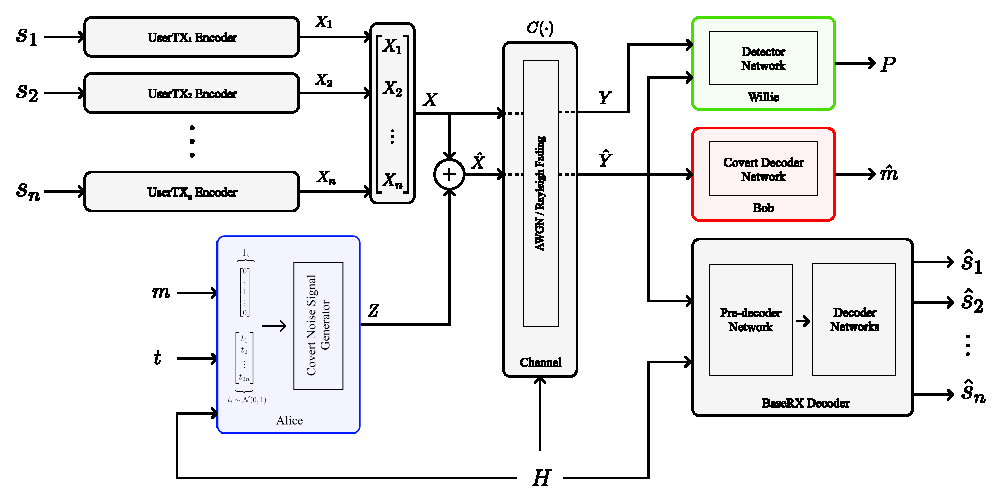
\includegraphics[width=\linewidth]{figs/multi_system_architecture}
	\end{subfigure}
	\\
	\caption{Overall architecture of our system model in the single-user scenario. Each UserTX uses its own encoder network to encode binary messages to a vector of signals and Alice perturbs them using her covert signals. After pass through the channel, BaseRX extracts the normal messages, Bob decodes the covert message, and Willie tries to distinguish covert and normal signals from the signals. (Colored components are under the control of covert users and gray components are the non-controllable parts of the system)}
	\label{fig:multi_system_architecture}
\end{figure*}

\section{GAN-Based Covert Model}
For a given binary secret message \(m\), Alice first one-hot encodes the message and then uses its generator model to produce a covert noise signal \(Z\). She then perturbs the ongoing normal signals \(X\) by adding this covert signal to them. Alice's generated covert signals are input-agnostic. That means her covert signals are produced independent of the \(X\) values. Hence, she requires no access to the content of \(X\) nor the message it carries. 

In the single-user scenario, we denote the final covet signal before being transmitted over the channel as:
\begin{equation}
	\hat{X} = X + Z.
\end{equation}

For the multi-user system, Alice perturbs all the signals at once using the same covert noise signal. Thus, the final covert signal for each transmitter is expressed as:
\begin{equation}
	\hat{X}_i = X_i + Z.
\end{equation}

This perturbed signal that embodies the covert signal within is then transmitted over the channel. As we mentioned before, we consider three channel models of AWGN, Rayleigh fading, and Rician fading. Therefore, there will be three different channel outputs for these three channel models. We use a mapping function \(\mathcal{C}(\cdot)\) to express each of these channels' outputs. Since signals in the multi-user system also undergo an extra channel effect called channel interference, we express single-user and multi-user channel's outputs separately.


\textit{AWGN Channel Output}: For the AWGN channel model, the signal received at the receiver carries within itself the channel's noise effect \(N \sim \mathcal{N}(0, \sigma^2)\). Thus, the channel function \(\mathcal{C}(\cdot)\) and the final covert signal \(\hat{y}\) in the single-use system can be represented as:
\begin{equation}
	\hat{Y} = \mathcal{C}(\hat{X}) = \hat{X} + N.
\end{equation}
For the multi-user system, signals also get distorted by the channel interference effect. This is due to the multiple transmitters sending their signals at the same time causing interference at the receiver's antennas. Consequently, the resulting noisy signals of each transmitter can be denoted as:
\begin{equation}
	 \hat{Y}_i = \mathcal{C}(\hat{X}_i) = \sum^{i \in U}\hat{X}_i + N_i.
\end{equation}
where \(U\) is the set that contains all transmitters.

\textit{Rayleigh and Rician Fading Channel Outputs}: For the Rayleigh and Rician fading channel models, we consider a flat-frequency block-fading channel where each vector of signals, which corresponds to a codeword, is assumed to be faded independently. Let \(H\) be the fading coefficient for the signal vector \(\hat{X}\), then the channel function \(\mathcal{C}(\cdot)\) and the final covert signal \(\hat{Y}\) in the single-user system is given by:
\begin{equation}
	\hat{Y} = \mathcal{C}(\hat{X}) = H \cdot \hat{X} + N.
\end{equation}

In the multi-user case, the final covert including the channel interference can be written as:
\begin{equation}
	\hat{Y}_i = \mathcal{C}(\hat{X}_i) = \sum^{i \in U}(H_i \cdot \hat{X}_i) + N_i.
\end{equation}


On the receiver side, Bob receives the transmitted signal \(\hat{Y}\) that is distorted by the channel noise effect and also by the channel interference effect in the multi-user case. Using his decoder network, he reconstructs the covert message \(\hat{m}\). Meanwhile, the UserRX uses the same signal to extract the normal message \(\hat{s}\), which is the reconstructed version of the message \(s\).


The statistical properties of signals transmitted over the channel are captured by the Willie's substitute. This network's objective is to classify sequences of normal \(Y\) and covert signals \(\hat{Y}\) and provide useful feedback to Alice during training. This feedback helps Alice modify the produced covert signals such that they are indistinguishable from the normal transmitted signals so that later when model is deployed in a real communication setup, it is ensured that it will be highly unlikely for the system's observer to detect the covert transmissions. In other words, it guarantees the covertness by requiring both normal and covert signals to have similar statistical properties.

\subsection{General Formulation}

\textbf{Reliability}: The very first objective of our covert model is to have a working covert communication. To this end, Bob has to have a plausible accuracy in decoding covert messages that Alice sends through the covert signals \(\hat{Y}\). As mentioned earlier, Alice employs a generative model that generates covert noise signals that correspond to the covert messages. Having such a stochastic generative model for Alice results in each covert message getting mapped to a set of different covert noise signals instead of one. Let \(\Theta_{\mathcal{A}}(\cdot)\) be the underlying function of Alice's generative model that takes a random trigger \(t \sim \mathcal{N}(0, 1)\) and a covert message \(m\) and produces a covert signal \(Z\) (the corresponding covert signal then can be denoted as \(Z_{m, t} = \Theta_{\mathcal{A}}(m, t)\)). Let also  \(\Theta_{\mathcal{B}}(\cdot)\) be the underlying function of the decoder network that Bob utilizes to reconstruct the covert message \(\hat{m}\). Then the reliability of communication between Alice and Bob is achieved using the below loss function:
\begin{equation}
	\begin{aligned} \label{bob_loss}
	\mathcal{L}_{\mathcal{B}} & = \mathbb{E}_{m}[\mathcal{H}(\hat{m}, m)] \\
	& = \mathbb{E}_{m}[\mathcal{H}(\Theta_{\mathcal{B}}(\hat{Y}), m)] \\ 
	& = \mathbb{E}_{m}[\mathcal{H}(\Theta_{\mathcal{B}}(\mathcal{C}(\hat{X}), m)] \\ 
	& = \mathbb{E}_{m}[\mathcal{H}(\Theta_{\mathcal{B}}(\mathcal{C}(\Theta_{\mathcal{A}}(m, t) + X)), m)].
	\end{aligned}
\end{equation}


where \(\mathcal{H}(\cdot)\) is the cross entropy between the probability of reconstructed covert message \(\hat{m}\) and the actual covert message \(m\). This equation can be used for optimizing both Alice's and Bob's networks by freezing one or the other's network parameters iteratively. 

\textbf{Low Interference}: While (\ref{bob_loss}) ensures the communication accuracy, we also need to verify that the generated perturbations leave no detrimental impact on the normal communication between UserTX and UserRX, otherwise, any unexpected increase in the communication's error rate can be deemed as an abnormal behavior by Willie. To this end, in the single-user system, we impose this constraint by minimizing the UserRX's loss function during Alice's training:
\begin{equation}
	\begin{aligned} \label{alice_user_loss}
	\mathcal{L}_{\mathcal{U}} & = \mathbb{E}_{m}[\mathcal{H}(\hat{s}, s)] \\
	& = \mathbb{E}_{m}[\mathcal{H}(\Theta_{\mathcal{U}}(\hat{Y}), s)] \\
	& = \mathbb{E}_{m}[\mathcal{H}(\Theta_{\mathcal{U}}(\mathcal{C}(\hat{z} + X)), s)] \\
	& = \mathbb{E}_{m}[\mathcal{H}(\Theta_{\mathcal{U}}(\mathcal{C}(\Theta_{\mathcal{A}}(m, t) + X)), s)].
	\end{aligned}
\end{equation}
where \(\Theta_{\mathcal{U}}(\cdot)\) is UserRX's decoder network function. Note that UserRX's decoder network is frozen during this training and only Alice's parameters will get updated.

For the multi-user system, since we have multiple transmitters sending signals, we need to minimize the BaseRX's loss function over all individual transmitters' signals. Thus, equation \ref{alice_user_loss} is rewritten as:
\begin{equation}
	\begin{aligned} \label{multi_alice_user_loss}
		\mathcal{L}_{\mathcal{U}} & = \sum^{i \in U}\mathbb{E}_{m}[\mathcal{H}(\hat{s}_i, s_i)] \\
		= \sum^{i \in U} & 
		\begin{cases} 
			\mathbb{E}_{m}[\mathcal{H}((\Theta_{\mathcal{U}}(\mathcal{C}((\Theta_{\mathcal{A}}(m, t) +  X_i)), s_i)] & AWGN \\
			\mathbb{E}_{m}[\mathcal{H}((\Theta_{\mathcal{U}}(\mathcal{C}((\Theta_{\mathcal{A}}(m, t, h) + X_i), h), s_i)] & Rayleigh. \\
		\end{cases} 
	\end{aligned}
\end{equation}

\begin{algorithm}[tp!]
	\caption{Optimizing covert models algorithm}\label{alg:cap}
	\small
	\begin{algorithmic}
		\State $X \gets$ normal signals data
		\State $S, M \gets$ normal and covert messages sets
		\State $\Theta_{\mathcal{A}}, \Theta_{\mathcal{B}}, \Theta_{\mathcal{W}} \gets$ Alice, Bob, and Willie network functions
		\State $\Theta_{\mathcal{U}} \gets$ UserRX decoder network function
		\State $\mathcal{H} \gets$ cross entropy function
		\State $\mathcal{C} \gets$ channel mapping function
		\For{epoch $ep \in \{1 \ldots n_{epochs}$\}}
		\State $t \sim \mathcal{N}(0, 1)$
		\State $\mathcal{L}_{\mathcal{W}} = \mathcal{H}(\mathcal{C}(X), \mathcal{C}(\Theta_{\mathcal{A}}(M, t) + X))$
		\State Update $\Theta_{\mathcal{W}}$ to minimize $\mathcal{L}_{\mathcal{W}}$
		\State $\mathcal{L}_{\mathcal{B}} = \mathcal{H}(\mathcal{C}(\Theta_{\mathcal{A}}(M, t) + X), M)$
		\State Update $\Theta_{\mathcal{B}}$ to minimize $\mathcal{L}_{\mathcal{B}}$
		\State $\mathcal{L}_{\mathcal{U}} \gets \mathcal{H}(\Theta_{\mathcal{U}}(\mathcal{C}(\Theta_{\mathcal{A}}(M, t) + X)), S)$
		\State
		$\mathcal{L}_{\mathcal{A}} = \lambda_{\mathcal{B}} \mathcal{L}_{\mathcal{B}} + \lambda_{\mathcal{U}} \mathcal{L}_{\mathcal{U}} - \lambda_{\mathcal{W}} \mathcal{L}_{\mathcal{W}}$
		\State Update $\Theta_{\mathcal{A}}$ to minimize $\mathcal{L}_{\mathcal{A}}$
		\EndFor
	\end{algorithmic}
\end{algorithm}

\textbf{Undetectability}: In our model, we employ a critic network, similar to what is known as a discriminator in GAN models \cite{goodfellow2014generative}, to serve as the Willie's detection network substitute. The so-called real and fake samples in GANs' discriminator network training process here are mapped to normal and covert signals, respectively. That is, for the single-user system we use the below loss function to optimize Willie's subtitle network to classify covert and normal signals:
\begin{equation}
	\begin{aligned} \label{willie_loss}
	\mathcal{L}_{\mathcal{W}} & = \mathbb{E}_{m}[\mathcal{H}(\hat{y}, y)] \\
	& = \mathbb{E}_{m}[\mathcal{H}(\mathcal{C}(\hat{X}), \mathcal{C}(X))] \\
	& = \mathbb{E}_{m}[\mathcal{H}(\mathcal{C}(\Theta_{\mathcal{A}}(m, t) + X), \mathcal{C}(X))].
	\end{aligned}
\end{equation}
where \(\mathcal{H}(\cdot)\) is the binary cross entropy between the covert signals \(\hat{Y}\) and the normal signals \(Y\). 

And again for the multi-user system, we need to optimize the Willie's subtitle network over all the transmitters' outputs.

\begin{equation}
	\begin{aligned} \label{multi_willie_loss}
		\mathcal{L}_{\mathcal{W}} & = 
		\sum^{i \in U} \mathbb{E}_{m}[H(\hat{Y}, Y)] \\
		= \sum^{i \in U} & = \begin{cases}
			\mathbb{E}_{m}[\mathcal{H}(\mathcal{C}(\Theta_{\mathcal{A}}(m, t) + X), \mathcal{C}(X))] & AWGN \\
			\mathbb{E}_{m}[\mathcal{H}(\mathcal{C}(\Theta_{\mathcal{A}}(m, t, H) + X), \mathcal{C}(X))] & Rayleigh.
		\end{cases}
	\end{aligned}
\end{equation}

This white-box adversarial training against Alice's network ensures that the Willie's substitute network will be adequately trained to tell covert and normal signals apart. On the other hand, we do not want the covert signals that Alice produces to deviate from the statistical properties of the normal signals on the channel, otherwise it is likely that the observer of the channel detects and mitigates the covert communication. To achieve this undetectability property, we utilize this network to perform what discriminator networks do in GAN setups in Alice's optimization function. In other words, Alice training against this network results in maximizing Willie's uncertainty about his predictions and having a regularizer as such helps Alice and Bob to form their covert communication in a way that is indistinguishable from the actual channel's noise, yet understandable by both. Altogether, Alice's loss function can be expressed as a weighted sum of these three objectives:
\begin{equation}
	\begin{array}{l} \label{alice_loss}
	\mathcal{L}_{\mathcal{A}} = \lambda_{\mathcal{B}} \mathcal{L}_{\mathcal{B}} + \lambda_{\mathcal{U}} \mathcal{L}_{\mathcal{U}} - \lambda_{\mathcal{W}} \mathcal{L}_{\mathcal{W}}.
\end{array}
\end{equation}
where \(\lambda_{\mathcal{B}}\), \(\lambda_{\mathcal{U}}\), and \(\lambda_{\mathcal{W}}\) determine the importance of Alice's objectives. Algorithm \ref{alg:cap} summarizes the procedure by which we train our covert models.

\subsection{Neural Network Architecture}
\textbf{User's Autoencoder Network}: Autoencoder model accepts a binary message \(s\) of size \(k\) bits and outputs a reconstructed version of it \(\hat{s}\). Figure \ref{fig:autoencoder_architecture} depicts the overall architecture of our autoencoder model. The encoder part of the model first one-hot encodes the message and then maps it to a vector of signals of size \(2 \times n\), where \(n\) is the number of channel uses. In the case of multi-user system, there are multiple encoders involved. Thus, resulting vector will be of size \(n_{tx} \time 2 \times n\). These signals are then given to a mapping function that applies the channel noise and interference effects. On the receiver side, in the single-user system, two layers of parameter estimation and transformation only become active if the channel model is Rayleigh or Rician fading. In the single-user system, we consider a simple transformation function that divides the received signal by the channel fading coefficients estimated by the parameter estimation layer. Note that more complex transformation functions can be used and are described in \cite{o2017introduction}, however optimizing the performance of the autoencoder model is out of the scope of this article. In the multi-user system, channel coefficients are given as an input to the decoder. Thus, BaseRX equalizes the received signals using zero-forcing technique \cite{garg2010wireless}. In the single-user system, UserRX eventually reconstructs the message using its decoder network. In the multi-user system, BaseRX receives signals from all the transmitters at once and decodes them simultaneously by first passing the signals to a pre-decoder network and then using separate decoders at the ending layers.


\textbf{Alice's Network}: Similar to Autoencoder's encoder network, Alice takes a covert message \(m\) and transforms it to its corresponding one-hot encoding representation of it so that each message belongs to a unique class. Like any other generative model, Alice also needs a random trigger \(t\) to randomize the process by which the covert noise signal \(\hat{z}\) is produced. In the case of multi-user system, she receives the channel's matrix as an extra parameter. She then adds this covert signal to a normal signal \(x\) that is being transmitted at the time. When system has multiple users, she adds the same covert signal to all the transmitters' signals at once. For Alice's generator model, we use multiple dense layers with ReLU and Tanh activation functions. The first layer of this model takes a trigger random vector \(t\) and a one-hot encoded covert message \(m\), and an extra parameter \(h\) in the case of multi-user systems. This layer acts as an embedding layer by enlarging the input's domain space. The following fully connected layers are to extract the useful features and do the encoding process. The last layer of this model does a dimension transformation so that the generated covert signal \(\hat{z}\) complies with the dimension of the normal signal \(x\) on the channel. 


\textbf{Bob's Network}: Bob receives this covert signal \(\hat{y}\) that has undergone the channel's effects and feeds it through its decoder network and extracts the secret message by doing classification on the signal. Bob's network has a more complicated structure compared to Alice's as it has to decode the secret message from a distorted signal \(\hat{y}\) that has gone through the channel. The received message by Bob first goes through the first layer of the network, which is a dense layer wider than the input's followed by a Tanh activation function, to increase the input's feature space. Then the data is passed through multiple 1-Dimensional Convolutional (1D Conv) layers that learn the coding that Alice has established to encode the covert messages. We find that using 1D Conv layers helps Bob and Alice achieving a better consistency in the accuracy of their communication, especially when the channel model is more complicated (i.e., when there is also fading in the channel). The rest of Bob's decoder network consists of two dense layers that do a domain remapping from the learned feature space to the covert message domain space. Similar to the UserRX's and BaseRX's decoder networks, Bob eventually predicts the covert message by doing a classification on the received signal.


\textbf{Willie's Network}: Willie receives both the covert signal \(\hat{y}\) and the normal signal \(y\) and outputs a confidence probability \(P\) on how probable it is for the signal to be normal. We choose the same network architecture as Bob's for Willie except for the last layer that has a Sigmoid activation function instead of Softmax. Using the same network for both ensures Bob and Willie will have the same capacity of training and can compete each other in a fair setup.